%%%%%%%%%%%%%%%%%%%%%%%%% Packages
\documentclass[]{article}
\usepackage{authblk}
\usepackage[utf8]{inputenc}
\usepackage[english]{babel}
\usepackage{graphicx}
\usepackage{calligra}
\usepackage{gensymb}
\usepackage{float}
\usepackage{siunitx}
\usepackage{amsmath}
\usepackage{grffile}
\usepackage[mathscr]{euscript}
\usepackage{multicol}
\usepackage[document]{ragged2e}
\usepackage[margin=1.0in]{geometry}
\setlength{\parskip}{0.25em}
\renewcommand{\baselinestretch}{0.25}
%%%%%%%%%%%%%%%%%%%%%%%%% Document Info
\title{\textbf{Raman Spectroscopy}}
\author{Taylor Larrechea}
\affil{Colorado Mesa University}
\affil{Department of Physical and Environmental Sciences}
\date{February 18, 2019}
\begin{document}
\maketitle
%%%%%%%%%%%%%%%%%%%%%%%%% Abstract
\begin{abstract}
\paragraph{}
\setlength{\parskip}{1em}
The purpose of this article is to report the results of photon intensity and relative wavenumber for the Raman Scattering. This experiment that was conducted for this report used Titanium dioxide to observe the Raman Scattering. It was discovered that Titanium dioxide has relative wavenumbers and intensities that are similar in magnitude for both the anti-stokes and stokes' lines found in this experiment.
\end{abstract}
%%%%%%%%%%%%%%%%%%%%%%%%% Background
\section{Background}
\begin{multicols}{2}
\paragraph{}
\setlength{\parskip}{1em}
To begin to understand the results of this report, the Raman Scattering must first be explained. To be exact, Raman Scattering is the scattering of photons via molecules that are in higher energy levels [1]. There are two distinct areas (Ranges of relative wavenumbers) where this scattering effect can be observed. For this articles sake we will refer to the locations of these Raman Peaks, which are the locations of extremely high intensity that were observed using the Light Studio software, as both anti-Stokes and Stokes lines. The Stokes lines are lines of observed high intensity where the emitted photon has less energy and the material in which the photon is scattering into has more after this phenomena occurs [1]. The anti-Stokes lines are lines of observed high intensity where the emitted photon has more energy after scattering into the material where as the material has less after this happens [1]. The Stokes and anti-Stokes lines were both named after George Stokes who first observed this scattering effect in 1852 [1]. We will be focusing on these two scenarios throughout this experiment.
\end{multicols}
%%%%%%%%%%%%%%%%%%%%%%%%% Experimental Set-Up
\section{Experimental Set Up}
\begin{multicols}{2}
\paragraph{}
\setlength{\parskip}{1em}
The equipment used in this experiment consisted of mirrors, beam splitters, stands to hold these objects, a 90 milliwatt laser set and 785 nanometers, one Acton Spectropro SP-2300, and of course a computer and software to analyze the data. The software that was used to observe the Raman Scattering in this experiment was called Lightstudio. With the help of the Lightstudio we were able to export the data points to Excel where plots of these intensities and relative wavenumbers were created for this report. But before we can get to reporting the data that was found in this experiment we need to explain how the experiment was carried out. 
\paragraph{}
\setlength{\parskip}{1em}
After all the equipment is initially turned on, the laser from the 90 milliwatt source begins it journey to the Titanium dioxide sample that is suspended via a tray. The laser first contacts a mirror that redirects it in the vertical direction. After this first mirror, the laser then hits a another mirror where the direction and orientation of the laser is changed to be horizontal again. The purpose of these first two mirrors is to redirect the laser such that the light is traveling at a higher elevated distance off the table than when it initially began its path to the sample. The second mirror changes the direction to 90 degrees of the initial trajectory to where the light now will travel through a beam 70/30 beam splitter. This beam splitter takes out 70 percent of the light and redirects in a manner such that it hits a flat display so that the intensity of the light is cut down a bit. After the light from the laser travels through the beam splitter it hits another mirror where the light goes from a horizontal trajectory to a vertical one once again. After this mirror, the light travels through a focusing knob to help direct the light to a single point on the Titanium dioxide sample. After the light hits the Titanium dioxide sample, it begins it path to the spectrometer via the same path with a couple differences. After the light travels up through the focusing knob it hits the mirror that sits above it. The light then shifts to a horizontal direction and hits the beam splitter where as now the light is redirected towards the spectrometer. After this beam splitter the light can be analyzed with the use of the spectrometer and the CCD that is attached to it. The sample can now be analyzed with the assistance of Lightstudio.
\end{multicols}
%%%%%%%%%%%%%%%%%%%%%%%%% Procedure
\section{Procedure}
\begin{multicols}{2}
\paragraph{}
\setlength{\parskip}{1em}
After the experiment was initially set up, the collecting of data could begin. The first step in collecting the data in this experiment once all the equipment was setup was to start up Lightstudio. Settings inside this program had to be optimized for the laser and the spectrometer for the data to be worth reporting. These settings include binning the data, making sure it outputs to the correct folder and in the right format, as well as setting the wavelength for the laser. In our experiment the wavelength that was needed to be used in this experiment was 785 nanometers. Small perturbations from this number cause discrepancies in the data and makes it unreliable. Once the settings in Lightstudio were optimized for the experiment, the collecting of the data could finally begin. 
\paragraph{}
\setlength{\parskip}{1em}
The second step in collecting data was choosing a good time interval for capture time from the CCD. It was thought of at first that longer capture times (Such as ten seconds and longer) would be more efficient at reporting accurate data for the Stokes and anti-Stokes lines. On the contrary however it was found that shorter time intervals did just fine for capturing data. So in this experiment, the data that is reported came from time intervals of two seconds, three seconds, and four seconds. Anything shorter than two seconds caused very sporadic data that was not consistent and intervals after four seconds did not seem to improve with a longer time, as previously stated. 
\paragraph{}
\setlength{\parskip}{1em}
The third step in collecting data was choosing a relative wavenumber to focus to the spectrometer on. For starters, wavenumber and wavelength are similar but they are not the same thing. A wavenumber corresponds to how many waves fit in a given unit of measurement. For instance in this lab we were dealing with units of inverse centimeters. This essentially means the number that goes along with cm$^{-1}$ is the number of waves of light in one centimeter. The Stokes lines that were previously mentioned in the Background section are positive where as the anti-Stokes lines are negative. After the relative wavenumber was selected, the data could finally start to be collected.
\end{multicols}
%%%%%%%%%%%%%%%%%%%%%%%%% Results
\section{Results}
\begin{multicols}{2}
\paragraph{}
\setlength{\parskip}{1em}
Selecting the exposure time was the biggest factor in this experiment for the best results. As previously stated, the exposure times that were used in this experiment were two, three, and four seconds. Since the data was readily accessible for multiple runs, there are a total of two graphs for each exposure time (i.e two anti-Stokes and Stokes graphs corresponding to one exposure time). This was to ensure that the data would be more reliable rather than only using one data set. Figure 1 shows the data points for the anti-Stokes lines of Titanium dioxide in a two second interval.
%%%%%%%%%%%%%%%%%%%%%%%%% Figure 1
\begin{center}
    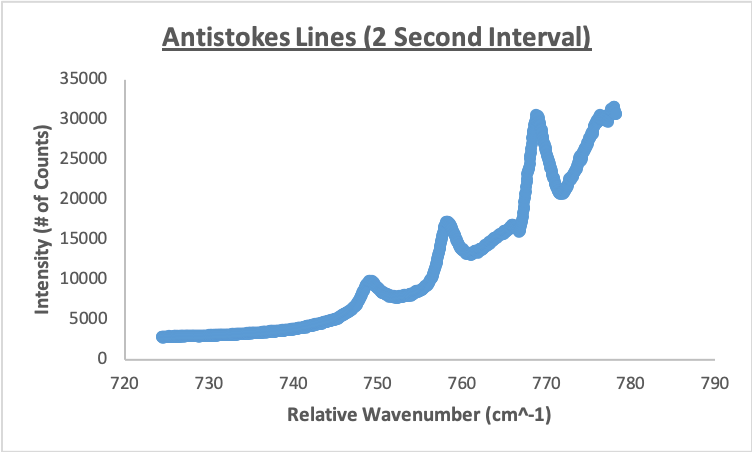
\includegraphics[width=7cm, height=4cm]{PHYS 331 RS (2 Sec) 1a.png}
    \caption{\textbf{\small{Figure 1: Anti-Stokes Lines at 2 Second Exposure Run 1.}}}
\end{center}
%%%%%%%%%%%%%%%%%%%%%%%%% Table 1
\begin{tabular}{|c|c|}
    \hline \textbf{Wavenumber (cm$^{-1}$)} & \textbf{Intensity (Counts)} \\ \hline
    749 & 2700 \\ \hline
    759 & 6000 \\ \hline
    769 & 14000 \\ \hline
\end{tabular}
\centerline{\tiny\textbf{{Table 1: Anti-Stokes Lines at 2 Second Exposure Run 1.}}}
\newline
Figure 1 and Table 1 both show the results of the 2 second exposure for the first run. The numbers that are displayed in the table for both the relative wavenumber and intensity are both estimates. The intensity is a lot more difficult to calculate due to the shape of the peaks that can be seen in Figure 1. Figure 2 shows the plot for the anti-Stokes lines at a two second exposure for a second time.
%%%%%%%%%%%%%%%%%%%%%%%%% Figure 2
\begin{center}
    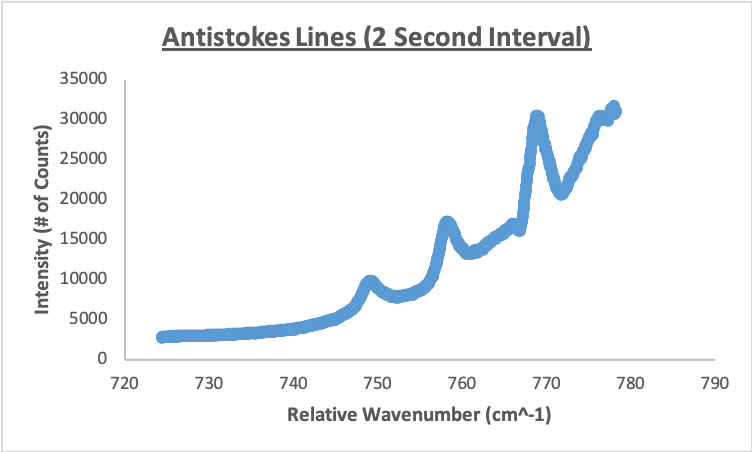
\includegraphics[width=7cm, height=4cm]{PHYS 331 RS (2 Sec) 1b.png}
    \caption{\textbf{\small{Figure 2: Anti-Stokes Lines at 2 Second Exposure Run 2.}}}
\end{center}
Figure 2 shows a pattern that is similar to that seen in Figure 1. This is as expected since the exposure time is the same. Table 2 shows the results in a numerical sense.
\newline
%%%%%%%%%%%%%%%%%%%%%%%%% Table 2
\begin{tabular}{|c|c|}
    \hline \textbf{Wavenumber (cm$^{-1}$)} & \textbf{Intensity (Counts)} \\ \hline
    750 & 2500 \\ \hline
    759 & 7000 \\ \hline
    769 & 14000 \\ \hline
\end{tabular}
\centerline{\tiny\textbf{{Table 2: Anti-Stokes Lines at 2 Second Exposure Run 2.}}}
\newline
The results that are found in Table 2 show that they are very similar to those found in Table 1. Now that the anti-Stokes lines have been reported the Stokes lines will now be examined. For the same two second time interval Figure 3 shows the plot of the Stokes lines of Titanium dioxide. 
%%%%%%%%%%%%%%%%%%%%%%%%% Figure 3
\begin{center}
    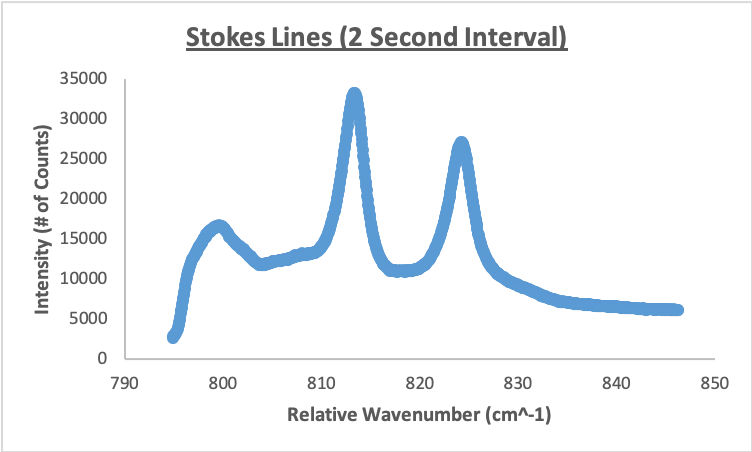
\includegraphics[width=7cm, height=4cm]{PHYS 331 RS (2 Sec) 2a.png}
    \caption{\textbf{\small{Figure 3:} Stokes Lines at 2 Second Exposure Run 1.}}
\end{center}
To look at the data found in Figure 3, Table 3 is created to make the results more clear.
\newline
%%%%%%%%%%%%%%%%%%%%%%%%% Table 3
\begin{tabular}{|c|c|}
    \hline \textbf{Wavenumber (cm$^{-1}$)} & \textbf{Intensity (Counts)} \\ \hline
    800 & 4500 \\ \hline
    814 & 14000 \\ \hline
    824 & 14000 \\ \hline
\end{tabular}
\centerline{\tiny\textbf{{Table 3: Stokes Lines at 2 Second Exposure Run 1.}}}
\newline
To have the most consistent data that we could possibly have, the same exposure time was ran again to have another data set to compare it to. Figure 4 shows the Stokes lines that were found with this same two second exposure.
%%%%%%%%%%%%%%%%%%%%%%%%% Figure 4
\begin{center}
    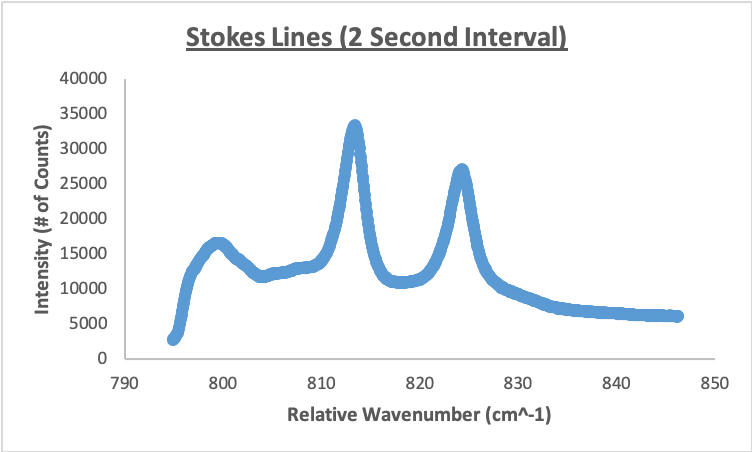
\includegraphics[width=7cm, height=4cm]{PHYS 331 RS (2 Sec) 2b.png}
    \caption{\textbf{\small{Figure 4:} Stokes Lines at 2 Second Exposure Run 2}}
\end{center}
We see that once again between the first and second run at the same exposure time that similar peaks arise. Table 4 has this data in a more concise manner.
\newline
%%%%%%%%%%%%%%%%%%%%%%%%% Table 4
\begin{tabular}{|c|c|}
    \hline \textbf{Wavenumber (cm$^{-1}$)} & \textbf{Intensity (Counts)} \\ \hline
    800 & 3500 \\ \hline
    814 & 15000 \\ \hline
    825 & 13000 \\ \hline
\end{tabular}
\centerline{\tiny\textbf{{Table 4: Stokes Lines at 2 Second Exposure Run 2.}}}
\newline
Figures 1-4 and Tables 1-4 depict the data that was collected for the exposure time of two seconds. Throughout the reporting of the data, the relative wavenumbers and intensities look to be similar to one another. Now the task is to change the exposure time to a different interval and compare the results.
\paragraph{}
\setlength{\parskip}{1em}
After the two second interval was completed, the three second interval was examined to compare results between one another. Figure 5 shows the anti-Stokes lines that were found for Titanium dioxide at a time exposure of three seconds.
%%%%%%%%%%%%%%%%%%%%%%%%% Figure 5
\begin{center}
    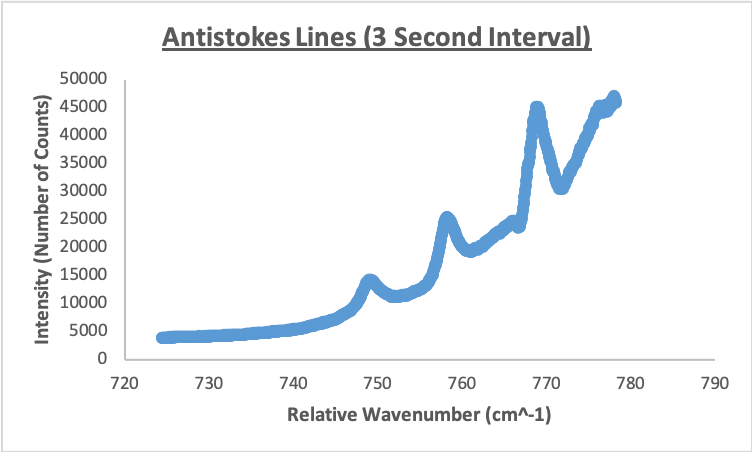
\includegraphics[width=7cm, height=4cm]{PHYS 331 RS (3 Sec) 1a.png}
    \caption{\textbf{\small{Figure 5:} Anti-Stokes Lines at 3 Second Exposure Run 1.}}
\end{center}
We can take this data and put it into a table that is seen in Figure 5. Table 5 shows this data.
\newline
%%%%%%%%%%%%%%%%%%%%%%%%% Table 5
\begin{tabular}{|c|c|}
    \hline \textbf{Wavenumber (cm$^{-1}$)} & \textbf{Intensity (Counts)} \\ \hline
    750 & 5500 \\ \hline
    759 & 7500 \\ \hline
    769 & 16000 \\ \hline
\end{tabular}
\centerline{\tiny\textbf{{Table 5: Anti-Stokes Lines at 3 Second Exposure Run 1.}}}
\newline
Data shown in Table 5 shows that the anti-Stokes lines are similar to those found in the first time exposure of two seconds. This same time interval of three seconds is then ran again to examine to anti-Stokes lines in Titanium dioxide. Figure 6 shows the plot of data.
%%%%%%%%%%%%%%%%%%%%%%%%% Figure 6
\begin{center}
    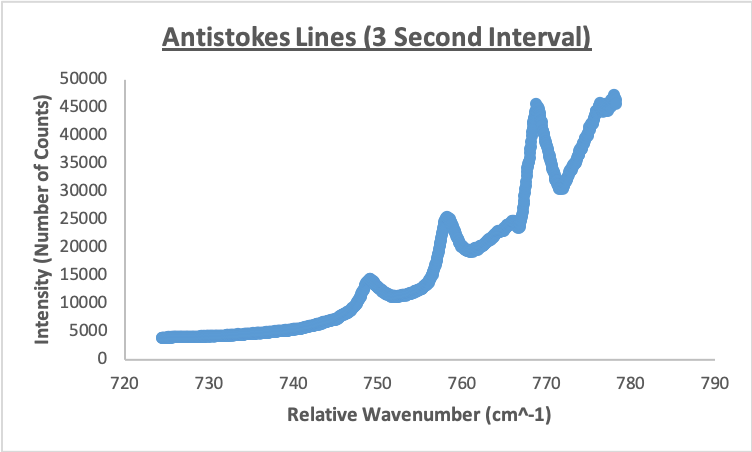
\includegraphics[width=7cm, height=4cm]{PHYS 331 RS (3 Sec) 2a.png}
    \caption{\textbf{\small{Figure 6:} Anti-Stokes Lines at 3 Second Exposure Run 2.}}
\end{center}
Once again it can be observed that Figure 5 and Figure 6 have the same shape of a plot for the Raman peaks. Comparing them to Figure 1 and Figure 2, Figure 6 is also consistent. Table 6 shows the data found in this new time interval.
\newline
%%%%%%%%%%%%%%%%%%%%%%%%% Table 6
\begin{tabular}{|c|c|}
    \hline \textbf{Wavenumber (cm$^{-1}$)} & \textbf{Intensity (Counts)} \\ \hline
    750 & 6000 \\ \hline
    759 & 6000 \\ \hline
    769 & 17000 \\ \hline
\end{tabular}
\centerline{\tiny\textbf{{Table 6: Anti-Stokes Lines at 3 Second Exposure Run 2.}}}
\newline
The data in Table 6 is correlating with Table 5 so we know that our data is reliable up to this point. Now the Stokes lines at the three second exposure time will be looked at. Figure 7 shows the Stokes lines for Titanium dioxide under a three second exposure. 
%%%%%%%%%%%%%%%%%%%%%%%%% Figure 7
\begin{center}
    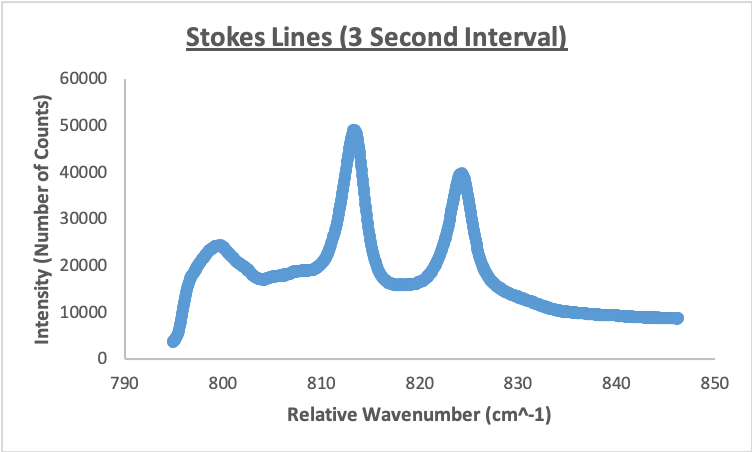
\includegraphics[width=7cm, height=4cm]{PHYS 331 RS (3 Sec) 1b.png}
    \caption{\textbf{\small{Figure 7:} Stokes Lines at 3 Second Exposure Run 1.}}
\end{center}
We can take the results from Figure 7 and put them into a table to get Table 7.
\newline
%%%%%%%%%%%%%%%%%%%%%%%%% Table 7
\begin{tabular}{|c|c|}
    \hline \textbf{Wavenumber (cm$^{-1}$)} & \textbf{Intensity (Counts)} \\ \hline
    800 & 4000 \\ \hline
    814 & 15000 \\ \hline
    825 & 14000 \\ \hline
\end{tabular}
\centerline{\tiny\textbf{{Table 7: Stokes Lines at 3 Second Exposure Run 1.}}}
\newline
We are continuing to have relative wavenumbers and intensities that are similar to one another regardless of the time interval that is used. We use the three second time interval one more time to examine the Stokes lines. Figure 8 shows the plot of the data.
%%%%%%%%%%%%%%%%%%%%%%%%% Figure 8
\begin{center}
    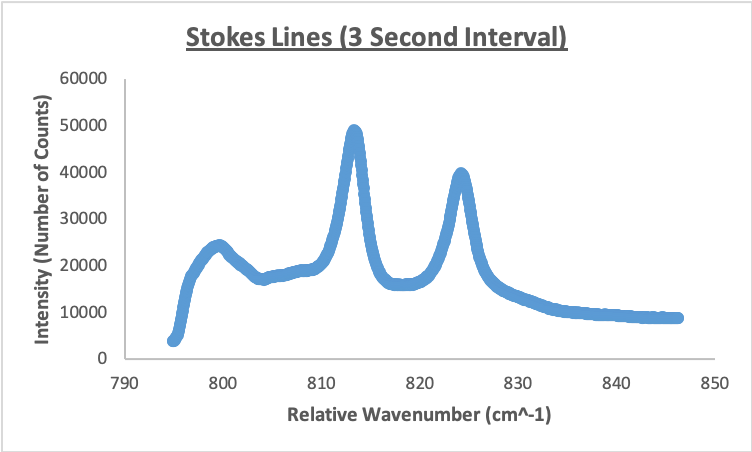
\includegraphics[width=7cm, height=4cm]{PHYS 331 RS (3 Sec) 2b.png}
    \caption{\textbf{\small{Figure 8:} Stokes Lines at 3 Second Exposure Run 2.}}
\end{center}
Figure 8 shows that the Stokes lines found in this exposure are consistent with the previous two second exposure that was used. This data is then examined to create Table 8 to have a more concise way to see the relative wavenumber and intensity at that wavenumber.
\newline
%%%%%%%%%%%%%%%%%%%%%%%%% Table 8
\begin{tabular}{|c|c|}
    \hline \textbf{Wavenumber (cm$^{-1}$)} & \textbf{Intensity (Counts)} \\ \hline
    800 & 4500 \\ \hline
    814 & 16000 \\ \hline
    825 & 13000 \\ \hline
\end{tabular}
\centerline{\tiny\textbf{{Table 8: Stokes Lines at 3 Second Exposure Run 2.}}}
\newline
We can see in both Figure 8 and Table 8 that this data is consistent with out previous results with only  discrepancies that are significant in the intensity. This now concludes the three second exposure time that was used to examine Raman Scattering.
\paragraph{}
\setlength{\parskip}{1em}
The last time interval that needs to be examined is the four second exposure time interval. Before the data was collected for these four second intervals it was assumed that this time exposure would be the best at recording reliable data. Figure 9 shows the anti-Stokes lines that were examined for this four second time exposure.
%%%%%%%%%%%%%%%%%%%%%%%%% Figure 9
\begin{center}
    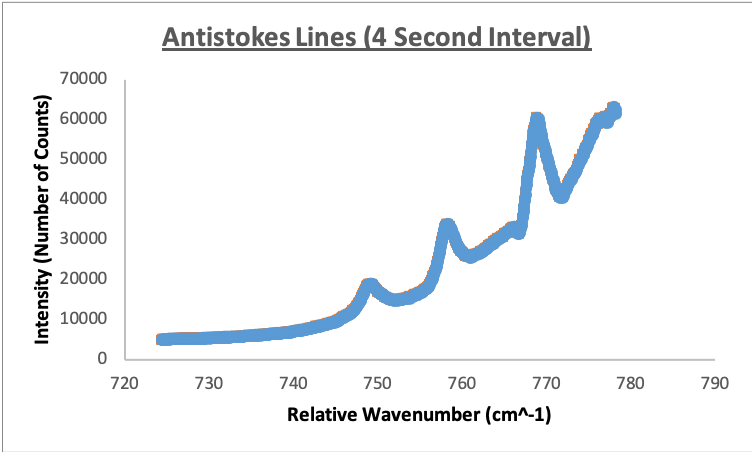
\includegraphics[width=7cm, height=4cm]{PHYS 331 RS (4 Sec) 1a.png}
    \caption{\textbf{\small{Figure 9:} Stokes Lines at 4 Second Exposure Run 1.}}
\end{center}
Figure 9 is reminiscent of the previous plots that depicted the anti-Stokes line of Titanium dioxide. When the data for these points were recorded with Lightstudio, it should be noted that these data sets (The exposure time of four seconds) had the smoothest curves on the plots within Lightstudio. Therefore these plots should be looked at as the primary results found in this experiment. Table 9 shows the data that was used to make the plot found in Figure 9.
\newline
%%%%%%%%%%%%%%%%%%%%%%%%% Table 9
\begin{tabular}{|c|c|}
    \hline \textbf{Wavenumber (cm$^{-1}$)} & \textbf{Intensity (Counts)} \\ \hline
    750 & 4500 \\ \hline
    759 & 7000 \\ \hline
    769 & 17000 \\ \hline
\end{tabular}
\centerline{\tiny\textbf{{Table 9: Anti-Stokes Lines at 4 Second Exposure Run 1.}}}
\newline
This data shows that these peaks occur at relatively high frequencies. Continuing on with reporting the data that was recorded for the four second exposure time, Figure 10 shows the plot of the anti-Stokes lines for Titanium dioxide once again.
%%%%%%%%%%%%%%%%%%%%%%%%% Figure 10
\begin{center}
    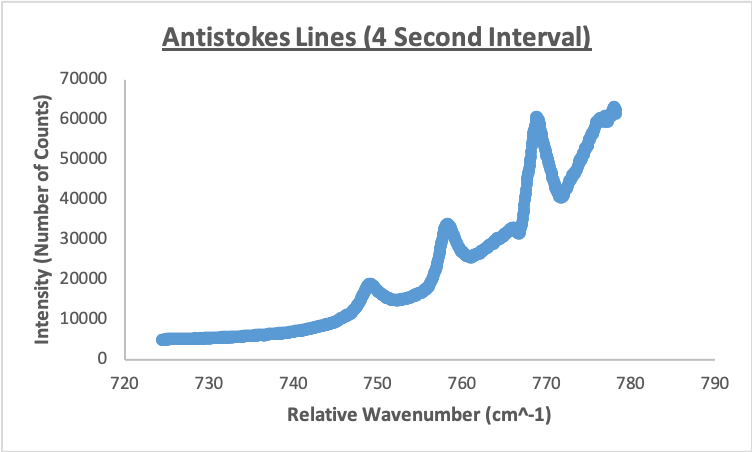
\includegraphics[width=7cm, height=4cm]{PHYS 331 RS (4 Sec) 2a.png}
    \caption{\textbf{\small{Figure 10:} Anti-Stokes Lines at 4 Second Exposure Run 2.}}
\end{center}
Figure 10 shows solidifies our results for what we see as the anti-Stokes lines that were present in the Titanium dioxide sample. Table 10 is then created to help clarify what is observed to be the relative wavenumber and intensity.
\newline
%%%%%%%%%%%%%%%%%%%%%%%%% Table 10
\begin{tabular}{|c|c|}
    \hline \textbf{Wavenumber (cm$^{-1}$)} & \textbf{Intensity (Counts)} \\ \hline
    750 & 4000 \\ \hline
    759 & 7000 \\ \hline
    769 & 17000 \\ \hline
\end{tabular}
\centerline{\tiny\textbf{{Table 10: Anti-Stokes Lines at 4 Second Exposure Run 2.}}}
\newline
We can now see with the aide of Figure 10 and Table 10 that the anti-Stokes of Titanium dioxide with the laser centered $\pm$ 561 nm are somewhere around 750, 759, and 769 cm$^{-1}$. The last two Figures and Tables pertain to the Stokes lines of the Titanium dioxide sample at four seconds exposure. With this we now have Figure 11.
%%%%%%%%%%%%%%%%%%%%%%%%% Figure 11
\begin{center}
    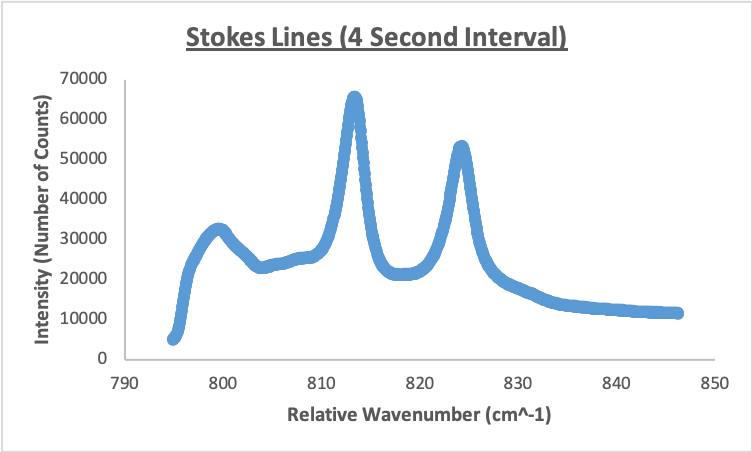
\includegraphics[width=7cm, height=4cm]{PHYS 331 RS (4 Sec) 1b.png}
    \caption{\textbf{\small{Figure 11:} Stokes Lines at 4 Second Exposure Run 1.}}
\end{center}
Figure 11 is also reminiscent of the previous plots that depicted the Stokes line of the Titanium dioxide sample. With the intention of identifying the relative wavenumbers of this Titanium dioxide sample, Table 11 is created to help relay the data. 
\newline
%%%%%%%%%%%%%%%%%%%%%%%%% Table 11
\begin{tabular}{|c|c|}
    \hline \textbf{Wavenumber (cm$^{-1}$)} & \textbf{Intensity (Counts)} \\ \hline
    800 & 7000 \\ \hline
    814 & 27000 \\ \hline
    825 & 25000 \\ \hline
\end{tabular}
\centerline{\tiny\textbf{{Table 11: Stokes Lines at 4 Second Exposure Run 1.}}}
\newline
When the exposure time was increased for observing the Stokes lines, the intensity of the Titanium dioxide sample went up. Instead of being around the previous values that were found in Tables (3-4) and (7-8), these values were almost double of what was observed before. This may be largely in part due to the exposure time being just enough longer for a significant amount more photons to enter the detector. The last figure that is to be reported for this observation of the Raman Scattering is Figure 12. Figure 12 shows the last run for the four second exposure of the Stokes lines in the Titanium dioxide sample.
%%%%%%%%%%%%%%%%%%%%%%%%% Figure 12
\begin{center}
    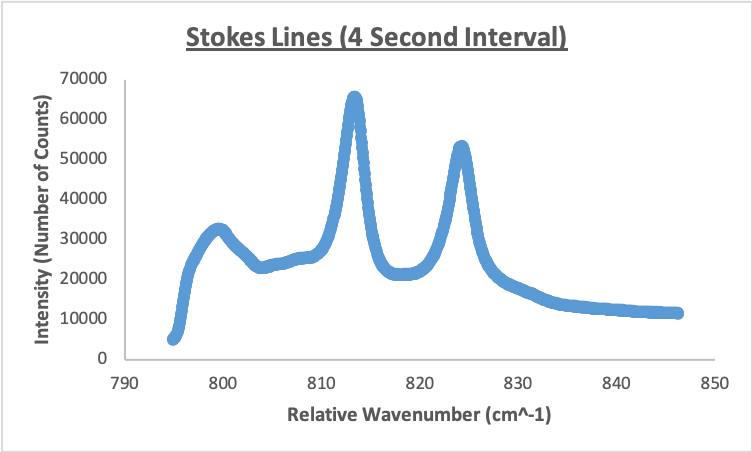
\includegraphics[width=7cm, height=4cm]{PHYS 331 RS (4 Sec) 1b.png}
    \caption{\textbf{\small{Figure 12:} Stokes Lines at 4 Second Exposure Run 2.}}
\end{center}
Figure 12 shows results that are similar to that seen in Figure 11. This helps solidify what we should expect to see for the stokes lines in Titanium dioxide centered at the 589 cm$^{-1}$ wavenumber. Table 12 relays the data for the relative wavenumbers and intensities one last time for Titanium dioxide seen in Figure 12.
\newline
%%%%%%%%%%%%%%%%%%%%%%%%% Table 12
\begin{tabular}{|c|c|}
    \hline \textbf{Wavenumber (cm$^{-1}$)} & \textbf{Intensity (Counts)} \\ \hline
    800 & 7000 \\ \hline
    814 & 26000 \\ \hline
    825 & 25000 \\ \hline
\end{tabular}
\centerline{\tiny\textbf{{Table 12: Stokes Lines at 4 Second Exposure Run 2.}}}
\newline
Table 12 solidifies the relative wavenumber for the Stokes lines of Titanium dioxide. This concludes the data collection of this report.
\end{multicols}
%%%%%%%%%%%%%%%%%%%%%%%%% Conclusion
\section{Conclusion}
\begin{multicols}{2}
\paragraph{}
\setlength{\parskip}{1em}
Multiple tests were conducted to see what were the relative wavenumbers that the anti-Stokes and Stokes lines occurred at for Titanium dioxide. The first sets of tests were conducted at time intervals of only two seconds, to eventually three, and lastly four seconds. There were a total of six plots and tables for the anti-Stokes lines and another six plots and tables for the Stokes lines to try and get the most accurate results possible. Through trial and error it was discovered that the four second exposure time was the best exposure time for ensuring accurate data collection. This was because the collector had adequate time to collect data to where there was not any skipping in between the data points. Although it cannot be seen in the excel plots above, this skipping phenomena occurs a lot between the data points at the two second interval. This defect improves at the three second interval, but the four second reigns supreme for its accuracy of collecting data points. After all this we could say that our anti-Stokes lines for Titanium dioxide occur at 750, 759, and 769 cm$^{-1}$. The Stokes lines occur at 800, 814, and 825 cm$^{-1}$ according to our findings.
\end{multicols}
\newpage
%%%%%%%%%%%%%%%%%%%%%%%%% Bibliography
\begin{thebibliography}{1}
\bibitem{Wikipedia Raman Scattering}
Wikipedia. Wikipedia. 31 January 2019. 16 February 2019. <https://en.Wikipedia.org/wiki/Raman$_$scattering>.
\end{thebibliography}
\end{document}
